\documentclass[a4paper, 12pt,liststotoc]{scrartcl}
\usepackage{color}
\usepackage[T1]{fontenc}
\usepackage[utf8]{inputenc}
\usepackage{lmodern}
\usepackage[ngerman]{babel}
\usepackage{graphicx}
\usepackage{pdfpages}
\usepackage{booktabs}
\usepackage{tabularx}
\usepackage{tabulary}
\usepackage{longtable}
\usepackage{tikz}
\usepackage[hyphens]{url}
\usepackage{doi}
\usepackage[skip=2pt,font=small]{caption}
\usepackage{dcolumn}
\usepackage{lscape}
\usepackage{threeparttable}
\usepackage{array}
\clubpenalty=10000
\widowpenalty=10000
\displaywidowpenalty = 10000
\newcolumntype{L}[1]{>{\raggedright\arraybackslash}p{#1}}
\newcolumntype{C}[1]{>{\centering\arraybackslash}p{#1}}
\newcolumntype{R}[1]{>{\raggedleft\arraybackslash}p{#1}}
\usepackage[toc,page]{appendix}
\usepackage[style=authoryear,uniquename=false,natbib=true,backend=biber,url=false,isbn=false,doi=false]{biblatex}
\addbibresource{bib.bib}
\usepackage{setspace}
\usepackage{amsmath}
\numberwithin{equation}{section}
\onehalfspacing
\usepackage{csquotes}
\MakeOuterQuote{"}
\newcommand*{\source}[2]{%
  \caption[{#1}]{%
    #1%
    \\\hspace{\linewidth}%
    \scriptsize{\emph{Source:} #2}%
  }%
}
\newcommand*{\captionsource}[2]{%
  \caption[{#1}]{%
    #1%
    \\\hspace{\linewidth}%
    \\\hspace{\linewidth}%
    Quelle: #2%
    \\\hspace{\linewidth}%
  }%
}

\definecolor{Blue}{rgb}{.1,.1,.5}
\definecolor{Red}{rgb}{.5,.1,.1}
\definecolor{Gray}{rgb}{.8,.8,.8}
\parindent 0pt
\parskip 12pt

\begin{document}

\title{Erbschaftssteuerreform\thanks{Dank geht an Hans Frauchiger (Berner
  Steuerverwaltung) für die Arbeiten im Rahmen der Bereitstellung der Steuerdaten und Auskünfte zu steuertechnischen Details, an Ben Jann und
  Robert Fluder für wertvolle Hinweise, sowie an Jonas Meier für
  Recherchen und Unterstützung bei der Datenaufbereitung.}}
\subtitle{Auswertungen mit Berner Steuerdaten entlang der geplanten Reformen der eidgenössischen Volksinitiative "Millionenerbschaften besteuern für unsere AHV (Erbschaftssteuerreform)"}
\author{Oliver Hümbelin\thanks{Berner Fachhochschule, Fachbereich Soziale Arbeit, oliver.huembelin@bfh.ch} \and Rudolf Farys\thanks{Universität Bern, Institut für Soziologie, rudolf.farys@soz.unibe.ch}}
\date{\today}
\maketitle
\newpage

\begin{abstract}
Mit der Abstimmung über die eidgenössische Volksinitiative "Millionen-Erbschaften besteuern für unsere AHV (Erbschaftssteuerreform)" am 14. Juni 2015 rückte die Aufmerksamkeit betreffend der Vermögensverteilung und der Bedeutung von Erbschaften zunehmend ins öffentliche Interesse. Gleichzeitig ist der Wissenstand jedoch beschränkt. Dieser Kurzbericht begegnet dieser Wissenslücke auf der Basis von Steuerdaten des Kantons Bern (2002-2012). Auswertungen des Reinvermögens zeigen, dass die Vermögensverteilung sehr ungleich ist. Einige wenige besitzen sehr viel, während die Mehrheit über wenig verfügt und ein Teil sogar beträchliche Schulden aufweist. Entsprechend wären von einer Erbschaftssteuer auf Vermögen ab 2 Millionen nur sehr wenige betroffen (ca. 1,5 Prozent aller Steuersubjekte). Vererbt werden im Mittel jährlich 1,5 Milliarden; die Summe der jährlichen Schenkungen liegt etwas tiefer (1 Milliarde). Unserer Schätzung zu Folge würde die Steuer schweizweit ca. 1,07 Milliarden jährlich generieren. Gemäss Simulationen würde die Steuer nur sehr langsam Vermögen umverteilen.\footnote{Eine gekürzte Version dieser Studie wurde am 22 Mai 2015 unter dem Titel "Wer bei einem Ja zur Erb\-schafts\-steu\-er zahlen müsste" im Da\-ten\-blog von Ta\-me\-dia publiziert: \url{http://blog.tagesanzeiger.ch/datenblog/index.php/8754/so-viel-geld-wuerde-die-erbschaftssteuer-in-die-kasse-spuelen}}
\end{abstract}
\newpage

\tableofcontents
\newpage

\section{Erbschaftssteuer in der
Schweiz}\label{erbschaftssteuer-in-der-schweiz}

Die Besteuerung von Erbschaften ist international gesehen durchaus
üblich. Von den Industrieländern der OECD erheben lediglich Kanada und
Schweden keine Erbschaftssteuer und den Spitzenplatz hinsichtlich
Erbschaftssteuer belegt die USA mit einem Spitzensteuersatz von 55\%. Auch wenn im Zuge medialer Debatten ein anderer Eindruck entstehen
kann: Auch in der Schweiz werden bereits entsprechende Steuern erhoben.
Da die Kompetenzen dazu bei den Kantonen liegen, unterscheiden sich die
Verhältnisse jedoch kantonsweise stark. Entscheidend ist bei Erbgängen
der Verwandtschaftsgrad. Handelt es sich beim Erbempfänger um einen
Ehegatten, muss heute in keinem Kanton eine Erbschaftssteuer entrichtet
werden. Auch direkte Nachkommen (inkl. Adoptivkinder) sind mittlerweile
weitgehend von einer Erbschaftssteuer befreit. Einzig in Appenzell
Innerhoden, Waadt und Neuenburg werden Erbgänge an Kinder, Enkel,
Urenkel und Adoptivkinder nach wie vor besteuert. Inwiefern Eltern,
Grosseltern, Geschwister und andere Erbempfänger (etwa
Konkubinatspartner) besteuert werden, ist von Kanton zu Kanton
unterschiedlich geregelt. Erwähnenswert für die Schweiz ist
insbesondere, dass die Erbschaftssteuer an direkte Nachkommen in vielen
Kantonen erst im Zuge des Steuerwettbewerbes der letzten Jahre
abgeschafft wurde \parencite{estv2013}.

Die Erbschaftssteuerinitiative setzt bei der Vermutung an, dass der
Reichtum in der Schweiz zunehmend ungleich verteilt ist. Über eine
national geregelte Reform der Erbschafssteuer möchte das
Initiativekomitee einen Ausgleich schaffen. Im Kern beinhaltet die
Initiative folgende Punkte:

\begin{itemize}
\item
  Erbschaftssteuern durch die Kantone werden aufgehoben
\item
  Der Bund erhebt auf den Nachlass von natürlichen Personen und bei
  Schenkungen eine Steuer von 20 Prozent
\item
  Von der Steuer befreit ist

  \begin{itemize}
  \item
    Ein Freibetrag von 2 Millionen auf den Nachlass und alle
    steuerpflichtigen Schenkungen
  \item
    Der Teil, der dem Partner (Gatte, registrierter Partner) zugewendet
    wird oder von der Steuer befreiten juristischen Personen
  \item
    Geschenke von höchstens 20`000 CHF je Jahr und Person
  \end{itemize}
\end{itemize}

Das Initiativkomitee schlägt darüber hinaus vor, den steuerfreien Betrag
für Familienunternehmen und KMU's auf 50 Millionen zu erhöhen, überlässt
die Ausarbeitung jedoch dem Parlament.

Befürworter der Initiative argumentieren, dass Vererbung die
Ungleichverteilung von Vermögen festigt oder verstärkt. Gleichzeitig
wird moniert, dass mittels Erbnachlass das meritokratische Prinzip
untergraben wird und lediglich über Arbeit erwirtschaftetes Geld auch
verdientes Geld sei. Wohlstand auf Grund von Familienvermögen entspreche
dagegen einem feudalistischen Prinzip. Gegner der Initiative kritisieren
den staatlichen Eingriff in Angelegenheiten der Familie und empfinden
die mehrfache Besteuerung materieller Ressourcen als unverhältnismässig.
So wird bereits eine Steuer auf Einkommen erhoben; wird gespart, muss
weiter eine Steuer auf Vermögen entrichtet werden. Die Erbschaftssteuer
käme also einer Dreifachbesteuerung desselben Frankens gleich.
Gleichzeitig warnen die Kritiker vor einer allfällig schädigenden
Wirkung der Steuer, wenn etwa Betriebe verkauft werden müssen, um
gebundene Vermögenswerte für die Entrichtung der Steuer freizusetzen.

Gesicherte Informationen, anhand derer die Auswirkung der Steuer
beurteilt werden könnte, liegen jedoch wenig vor. Dieser Wissenslücke
möchten wir mit dem vorliegenden Bericht entgegenwirken und anhand einer
Auswertung von Steuerdaten des Kantons Bern aufzeigen, wie der Wohlstand
in Bern verteilt ist, wer von der Erbschaftssteuer betroffen wäre,
welche Summen in den letzten 10 Jahren verschenkt und vererbt wurden und
welche Steuersummen anhand einer Erbschaftssteuer generiert würden.
Abschliessen möchten wir den Bericht mit einer Simulation. Diese hat zum
Zweck zu untersuchen, wie stark die Erbschafssteuer effektiv zu einer
Umverteilung der Vermögen über die Zeit führt.

\section{Steuerdaten des Kantons
Bern}\label{steuerdaten-des-kantons-bern}

Im Rahmen des vom SNF finanzierten Projektes "Ungleichheit der Einkommen
und Vermögen der Schweiz" (\url{http://www.inequalities.ch}) wurden uns von der Berner
Steuerverwaltung Steuerdaten der Jahre 2002 -- 2012 zur Verfügung
gestellt. Diese umfassen ausführliche Informationen zur
Vermögenssituation von Steuersubjekten. Es lassen sich drei
Hauptvermögensarten unterscheiden:

\begin{itemize}
\item
  \emph{Finanzkapital:} Wertschriften, Guthaben, Bargeld, Gold und
  andere Edelmetalle
\item
  \emph{Liegenschaften:} Liegenschaften, Einfamilienhaus oder
  Stockwerkeigentum zum Verkehrswert besteuert sowie Land- oder
  Forstwirtschaft (zum Ertragswert besteuert)
\item
  \emph{Betriebsvermögen:} Betriebsvermögen Selbständigerwerbende
  (Geschäfts-/Be\-tei\-li\-gungs\-ka\-pi\-tal in Betrieben mit kaufm. Buchhaltung,
  Kunden- und andere Guthaben soweit im Wertschriftenverzeichnis nicht
  enthalten, Vorräte und Warenlager, Viehhabe, Anlagevermögen ohne
  Grundeigentum, z.B. Fahrzeuge, Maschinen/Mobiliar, Geräte, usw.)
\item
  \emph{Übriges Vermögen:} Lebens- und Rentenversicherungen,
  Motorfahrzeuge, Anteile an unverteilten Erbschaften,
  Geschäfts-/koorporationsanteile, übrige Vermögenswerte.
\end{itemize}

Zur Ermittlung des \emph{Reinvermögens} werden Schulden abgezogen.
Grundsätzlich können alle Schulden abgezogen werden, betragsmässig
fallen jedoch die Hypotheken auf Liegenschaften am stärksten ins
Gewicht. Für die nachfolgenden Auswertungen ziehen wir deshalb die Schulden vom Liegenschaftsvermögen ab.

Darüber hinaus werden in der Steuererklärung erhaltenes \emph{Erbe} und
erhaltene \emph{Schenkungen} erfasst. Ehegatten und Personen in eingetragener
Partnerschaft untereinander sowie Nachkommen, Stief- oder Pflegekinder
(mind. 2-jähriges Pflegeverhältnis) sind zwar von der Erbschafts- und
Schenkungssteuer befreit. Grössere Vermögensveränderungen, die für die
Steuerbehörde nicht nachvollziehbar sind, führen jedoch zu
Nachforschungen, weswegen die Angaben von Erben und Schenkungen in der
Regel auch in diesen Fällen vorhanden sind. Trotzdem ist davon
auszugehen, dass insbesondere kleinere Beträge z.T. nicht deklariert werden.

Anhand der Berner Steuerdaten ist es demnach möglich, verschiedene
Auswertungen zur geplanten Erbschaftssteuerreform vorzunehmen. Gegenüber
Befragungsdaten, die auf Stichproben beruhen, haben Steuerdaten den
Vorteil, dass Analysen auf eine Vollerhebung abgestützt werden können.
Es ist bekannt, dass Befragungen für Wohlstandsanalysen sehr
problematisch sind, weil sehr Reiche und sehr Arme in den Befragungen
nicht erreicht werden. Dies führt zu verzerrten Auswertungen. Mit diesen
methodischen Schwierigkeiten sind Steuerdaten nicht konfrontiert. Es
sind jedoch andere Restriktionen bekannt, die die Aussagekraft von
Vermögensanalysen mindern. Dazu gehören:

\begin{itemize}
\item
  Gesparte Vorsorgegelder (1. und 2. Säule) müssen nicht deklariert
  werden.
\item
  Liegenschaften sind unterbewertet, weil sie zum amtlichen und nicht
  zum Marktwert versteuert werden.
\item
  Steuerhinterziehung und Steueroptimierung: Mit zunehmendem Vermögen
  steigt der Anreiz Vermögenswerte vor dem Fiskus zu verbergen. Dazu
  gehören beispielsweise versteckte Konten und nicht deklarierte
  materielle Vermögenswerte (Kunst).
\item
  Steuereinheiten entsprechen nicht den realen Haushalten.
\end{itemize}

\section{Vermögensungleichheit, Erbschaften und potentielle
  Umverteilungswirkung der
  Erbschaftssteuer}\label{vermuxf6gensungleichheit-erbschaften-und-potentielle-umverteilungswirkung-der-erbschaftssteuer}
\subsection{Vermögensverteilung}\label{vermuxf6gensverteilung}

Im Jahr 2012 wurden im Kanton Bern Vermögen im Wert von 216 Milliarden
CHF deklariert. Die Vermögen im Kanton Bern sind damit fast so hoch wie
die jährliche Wirtschaftsleistung von ganz Griechenland (241 US-Dollar
Milliarden BIP). Wie sind diese Reichtümer verteilt? Zur Beurteilung der
Vermögenskonzentration lässt sich der Gini-Koeffizient berechnen. Mit
einem Wert von 0,78 liegt Bern schweizweit im Mittelfeld \parencite{jann2014}. In einigen Kantonen ist das Vermögen sehr viel stärker
konzentriert (beispielsweise Basel-Stadt und Genf) und in anderen
weniger (beispielsweise Uri). Weil der Gini-Koeffizient ein
Verteilungsmass mit vielen erwünschten statistischen Eigenschaften ist,
hat er sich in der Ungleichheitsforschung etabliert. Gleichzeitig führt
der Gini-Koeffizient zu einer Verdichtung der Information, die es
schwierig macht, den Charakter der Verteilung substantiell zu verstehen.
Deswegen zeigen wir die Verteilung des Wohlstandes in Bern mit
alternativen Indikatoren. Dafür werden die Steuersubjekte zunächst dem
Reinvermögen nach aufsteigend angeordnet und anschliessend in fünf
gleich grosse Gruppen eingeteilt. Es entstehen fünf Populationsquintile.
Q1 umfasst die 20 Prozent mit den geringsten Vermögen, Q2 die nächst
reicheren 20 Prozent etc. Q5 ist schliesslich die Gruppe der 20 Prozent
Reichsten.

\begin{figure}[!ht]
  \caption{Verteilung der Vermögen, Kanton Bern 2012}
  \label{fig:verteilung_vermoegen}
  \centering
    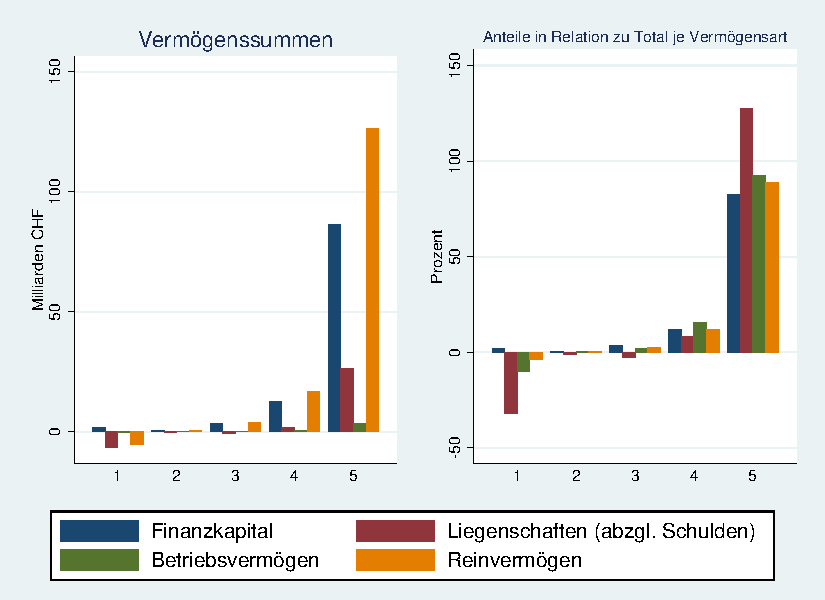
\includegraphics[width=\textwidth]{figure/VermoegenQuintil}
  \caption*{Quelle: Mikrosteuerdaten der Berner Steuerverwaltung, eigene Berechnungen}
\end{figure}

Nun kann berechnet werden, wie viel die jeweiligen Gruppen besitzen. Wir
zeigen dies aufgeschlüsselt für das Finanzkapital, die Liegenschaften
(abzüglich Schulden), das Betriebsvermögen und das Reinvermögen. Abbildung~\ref{fig:verteilung_vermoegen}
 zeigt, dass sich die Vermögen erheblich in der reichsten Gruppe
konzentrieren. D.h. die 20 Prozent Reichsten besitzen zusammen jeweils
an die 90 Prozent der jeweiligen Vermögenswerte, während die mittleren
Gruppen anteilmässig nur wenig besitzen und die ärmste Gruppe sogar
beträchtliche Schulden aufweist. Es fällt sofort auf, dass die reichsten
20 Prozent mehr als 100 Prozent bei den Liegenschaften besitzen. Dieses
im ersten Moment verwirrende Resultat ist jedoch auf die Schulden der
ärmsten 20 Prozent zurückzuführen. Ferner liegt Vermögen meist in Form von Finanzkapital oder
Liegenschaften vor. Auf der linken Seite der Abbildung ist gut ersichtlich,
dass es sich beim Betriebsvermögen um vergleichsweise kleine Summen
handelt.

Für die Erbschaftsteuerreform bedeutsam sind folgende Zahlen:

\begin{itemize}
\item
  Nur 9`166 Steuereinheiten verfügen über ein Reinvermögen von mehr als
  2 Millionen Franken und wären von der Steuer tangiert. Dies entspricht
  1,5 Prozent aller Steuersubjekte. Diese Gruppe besitzt 39 Prozent der
  gesamten Reinvermögen.
\item
  Betriebsvermögen von über 2 Millionen Franken liegen gemäss Angaben in
  den Steuerdossiers in 776 Fällen vor. Das maximale Betriebsvermögen
  liegt bei 43,3 Millionen Franken. Kein Betrieb käme demnach über der
  Grenze von 50 Millionen zu liegen, welche die Initiative für die
  Besteuerung vorsieht. Allerdings kann Betriebsvermögen auch Teil des
  privaten Finanzkapitals sein, wenn es in Form von Beteiligungen
  (Aktien, Anteile an GmbHs) vorliegt.
\end{itemize}

\subsection{ Erbschaften und Schenkungen
    }\label{erbschaften-und-schenkungen}

Wie sieht es nun mit Erbschaften und Schenkungen aus? In den letzten
zehn Jahren, wurden im Kanton Bern laut Daten der Steuerbehörden
jährlich im Mittel an die 1.5 Milliarden vererbt (siehe Abbildung~\ref{fig:schenkungen_und_erbe}) und etwas weniger
verschenkt (1.0 Milliarden Franken, ohne 2011). Auffällig sind die
Schenkungen im Jahr 2011. Diese Abweichung dürfte direkt auf die
Erbschaftsinitiative zurückzuführen sein. Die Initiative ist zwar erst
2013 zustande gekommen, bereits im Vorfeld wurde jedoch bekannt, dass
sie rückwirkend auf 2012 in Kraft treten soll. Dies gab offenbar Anlass,
vorbeugend Vermögen zu verschenken.

\begin{figure}[!ht]
  \caption{Schenkungen und Erbe, Kanton Bern 2002 -2012}
  \label{fig:schenkungen_und_erbe}
  \centering
    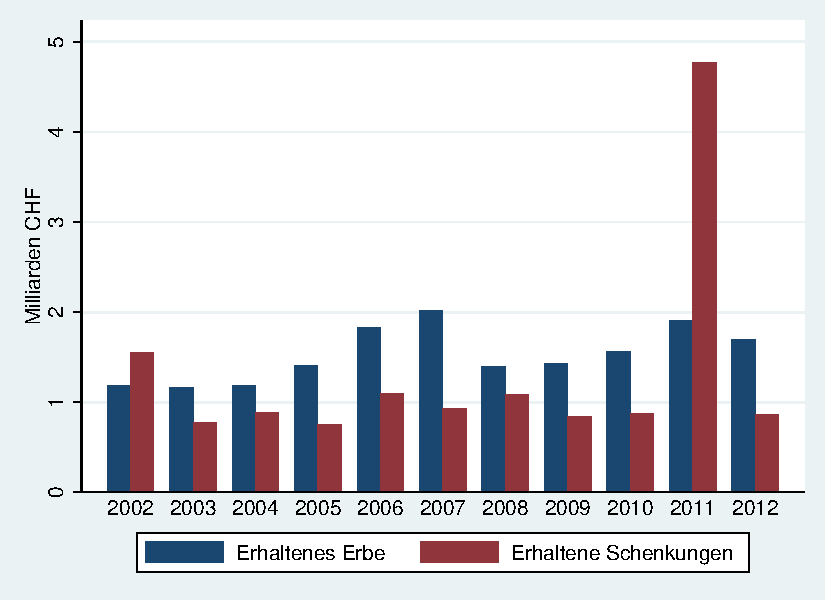
\includegraphics[width=\textwidth]{figure/ErbeSchenkungen}
  \caption*{Quelle: Mikrosteuerdaten der Berner Steuerverwaltung, eigene Berechnungen}
\end{figure}

Anhand der deklarierten Erbschaften und Schenkungen lässt sich
abschätzen, welches Steuervolumen damit hätte generiert werden können.
Dazu müssen wir einige Annahmen treffen, weil sich die Steuer laut
Initiativtext am Gesamtnachlass orientiert und nicht am erhaltenen
Betrag und wir aus den Steuerdaten lediglich die erhaltenen Beträge
kennen. Ebenso unbekannt bleibt der Verwandtschaftsgrad, der für die
Bestimmung der Steuerpflicht ausschlaggebend ist.

Weil im Erbfall in der Regel mehr als eine Person erbt, setzten wir die
Grenze der zu besteuernden Erbbeträge bei 1 Million an. Dies entspricht
der Annahme, dass immer genau zwei steuerpflichtige Personen erben.
Erbteile, die über 1 Million Franken hinausgehen, besteuern wir mit 20
Prozent. Je Jahr variiert so die berechnete Steuer erheblich. Das
Minimum beträgt 29,7 Millionen, das Maximum 156 Millionen und der Median
des Steuerbetrages ist 56 Millionen. Auch Schenkungen können wir
berücksichtigen. Dafür errechnen wir eine Steuer von 20 Prozent auf den
Teil von ausgerichteten Schenkungen, der 20`000 Franken überschreitet.
Weil Schenkungen bei einem Erblass an den Freibetrag von 2`000`000
angerechnet werden können, berechnen wir die Schenkungssteuer lediglich
für Steuersubjekte mit einem Reinvermögen über 2 Millionen. Im Mittel
kommen so je Jahr nochmals 48 Millionen hinzu (ohne 2011), also ähnlich
viel, wie aus der direkten Besteuerung der Erbschaften. 2011 wären
alleine auf Grund der Schenkungen 770,2 Millionen angefallen. Dies kommt
einem (hypothetischen) Steuerausfall von ca. 7 Jahren gleich.

Man kann sich nun die Frage stellen, welche Bedeutung diese Beträge für
das Staatsbudget haben. Im Schnitt wären mit der Erbschaftssteuer (inkl.
Schenkungen) Einnahmen von 104 Millionen je Jahr generiert worden Dies
entspricht immerhin drei Prozent des im Jahr 2012 über Einkommens- und
Vermögenssteuer durch natürliche Personen generierten Steuervolumens im
Kanton Bern. Anders ausgedrückt: würde die gesamte Summe dem Kanton Bern
zufallen, würde die Steuer das auf 2018 budgetierte Defizit von -72
Millionen des Berner Finanzplanes locker kompensieren, oder um näher am
Wunsch der Initianten zu bleiben (2/3 für die AHV und 1/3 für die
Kantone): der im Kanton Bern generierte Betrag entspräche 0.3 Prozent
der gesamtschweizerischen Jahresausgaben der AHV.

\subsection{Umverteilungswirkung der
Erbschafssteuer}\label{umverteilungswirkung-der-erbschafssteuer}

Weil die Erbschaftssteuer lediglich Vermögen über 2 Millionen besteuert,
hätte sie eine umverteilende Wirkung. Das heisst, finanzstarke Teile der
Bevölkerung werden stärker an den Kosten der öffentlichen Ausgaben
(Altersvorsorge, Verkehr, Bildung, Landesverteidigung etc.) beteiligt.
Die mit Steuergeldern bereit gestellten öffentlichen Güter können
wiederum von allen gleichermassen genutzt werden -- auch von
finanzschwachen Mitgliedern der Gesellschaft. Wenn wir einige (mutige)
Annahmen treffen, können wir simulieren, wie stark die Erbschaftssteuer
Vermögen von den Reichen zur Allgemeinheit umverteilt und damit der
ungleichen Verteilung der Vermögen entgegenwirkt, wie es das Ziel der
Erbschaftssteuerreform ist. Unteranderem nehmen wir dabei vereinfachend
an, dass ein durch die Steuer generierter Franken zu gleichen Teilen auf
die gesamte Bevölkerung (um)verteilt wird. Durch die Steuer werden also
Reichen ärmer und Arme reicher.

Ausgehend von der Vermögensverteilung 2012 zeigt der Umverteilungssimulator\footnote{\url{https://inequalities.shinyapps.io/simulation/}} 
in einer interaktiven Grafik, wie stark und in welchen Zeiträumen die
Erbschaftssteuer die bestehende Vermögensverteilung tangiert. Aus der
Grafik lässt sich erkennen, dass die betroffenen Vermögen etwa ein
Viertel der gesamten Vermögen ausmachen (bei einem Freibetrag von 2 Mio.
Franken). Bis diese mit einem Steuersatz von 20 Prozent verteilt sind,
vergeht eine sehr lange Zeit. Nach 30 Jahren ist die bestehende
Vermögensverteilung kaum verändert. Nach 350 Jahren sind zumindest die
Schulden der ärmsten 20 Prozent getilgt. Generell würden mit der
Erbschaftssteuer die Vermögen nur sehr langsam umverteilt. \href{https://inequalities.shinyapps.io/simulation/}{Finden Sie
selber heraus}, wie schnell sich die Vermögensverteilung ändert, wenn
etwa die amerikanische Version der Erbschaftssteuer Anwendung findet (3
Mio. Freibetrag und ein maximaler Steuersatz von 55 Prozent).

Unter der ambitionierten Annahme, dass keine legalen und illegalen Steuertricks zur Vermeidung einer Erbschaftssteuer angewandt werden (z.B. Umwandlung von Privat- in Betriebsvermögen, Kunstkauf, Nicht-Deklarieren von Vermögen), sind drei Parameter wichtig, um die Umverteilungswirkung der Steuer zu bestimmen. Die ersten beiden sind relativ offensichtlich: Der Freibetrag und der Steuersatz. Diese wurden in der Initiative mit 2 Millionen und 20 Prozent konzipiert. Der dritte und weniger offensichtliche Parameter ist die Dauer, bis ein und derselbe Franken erneut vererbt wird. Hieraus bestimmt sich, innerhalb welchen Zeitraums die 20 Prozent Steuern tatsächlich erhoben werden. Aus den Berner Steuerdaten können wir berechnen, dass pro Jahr etwa ein sechzigstel der Vermögen über 2 Millionen Franken vererbt oder verschenkt werden. Bis 20 Prozent der steuerbaren Masse besteuert wurden, vergehen demnach etwa 60 Jahre.  Wir nehmen weiter an, dass diese Steuereinnahmen gleichmässig auf die gesamte Bevölkerung verteilt werden. Der Rest der Verteilung wird als fix über die Zeit angenommen, d.h. die Simulation abstrahiert von potentiellen sonstigen Vermögensänderungen. Eine weitere implizite Annahme der Simulation ist, dass Vermögen nur innerhalb von Bern vererbt werden, bzw. Vermögen, die durch Vererbung den Kanton verlassen und solche, die dem Kanton zufliessen, sich gegenseitig aufheben.

\section{Fazit: Von der Erbschaftssteuer wären wenige
Betroffen}\label{fazit-von-der-erbschaftssteuer-wuxe4ren-wenige-betroffen}

Die Auswertung der Berner Steuerdaten zeigt dreierlei:

\begin{itemize}
\item
  Die Vermögen sind sehr ungleich verteilt. Obwohl die Steuerdaten die
  finanzielle Situation der gesamten Berner Bevölkerung detailliert
  abbilden, bleiben doch blinde Flecken. Nicht berücksichtigt werden
  können gesparte Vorsorgevermögen. Zwar ist davon auszugehen, dass die
  Ungleichverteilung mit den Vorsorgevermögen geringer ausfällt, es ist
  jedoch unbekannt, wie stark die Vorsorgevermögen in Relation zu den
  bestehenden Vermögenswerten ins Gewicht fallen. Gleichzeitig sind
  Vorsorgegelder zweckgebunden, und es ist fraglich, ob sie frei
  verfügbaren Mitteln gleichgesetzt werden können. Ferner
  unberücksichtigt bleiben jedoch auch undeklarierte Vermögenswerte
  (Steuerhinterziehung). Diese würden die Konzentration der Vermögen bei
  den Wohlhabendsten zweifelsfrei zusätzlich pointieren.
\item
  Entsprechend der Ungleichverteilung der Vermögen wären von der
  Erbschaftssteuerinitiative verhältnismässig wenige Personen betroffen.
  2012 verfügten 1,5 Prozent aller Steuerpflichtigen in Bern über ein
  Reinvermögen von mehr als 2 Millionen Franken und wären von der Steuer
  tangiert. Unten stehende Tabelle zeigt die Situation für die gesamte
  Schweiz im Jahr 2011 anhand der aktuellsten Vermögensstatistiken der
  Eidgenössischen Steuerverwaltung. Die Rangliste wird angeführt von
  Kantonen mit attraktiven Einkommens- und Vermögenssteuern für
  Wohlhabende (Schwyz, Zug, Nidwalden). Kein Muster ist zu erkennen,
  wenn auf Kantone fokussiert wird, die bereits jetzt eine
  Erbschaftssteuer direkter Nachkommen kennen (Appenzell Innerrhoden,
  Waadt und Neuenburg). Gesamtschweizerisch wären von der
  Erbschaftssteuer gut 100'000 Steuerpflichtige betroffen.
\item
  Ferner zeigen die Berner Steuerdaten, dass jährlich im Schnitt 1,5
  Milliarden veerbt und 1 Milliarde verschenkt wird. Damit lässt sich
  abschätzen, welche Steuersummen sich mit einer Erbschaftssteuer
  ergeben. In Bern würden im Schnitt jährlich an die 105 Millionen in
  die Staatskassen gespült. Setzt man die Berner Vermögen ins Verhältnis
  zum gesamtschweizerischen Vermögen, ergibt sich eine stolze Summe von
  1,07 Milliarden Franken.
\end{itemize}

\begin{table}
%\begin{longtable}[c]{@{}llll@{}}
\centering
\footnotesize
\caption{Steuerpflichtige mit Reinvermögen über 2 Mio, 2011}
\begin{tabular}{L{2.2cm}L{2.5cm}L{2.5cm}L{3cm}}
\toprule
~ & Anzahl & Anteil & Gesamtanzahl Steuerpflichtige\\
\midrule
SZ & 4774 & 5.2\% & 92184\\
ZG & 3461 & 5.1\% & 67849\\
NW & 1096 & 4.1\% & 26534\\
ZH & 27283 & 3.2\% & 861726\\
AI & 284 & 2.9\% & 9894\\
GE & 6314 & 2.4\% & 259980\\
AR & 741 & 2.2\% & 34234\\
BS & 2573 & 2.1\% & 124180\\
OW & 480 & 1.9\% & 24903\\
\midrule
Schweiz & 95943 & 1.9\% &
5006854\\
\midrule
VD & 7714 & 1.8\% & 418882\\
LU & 4142 & 1.8\% & 228890\\
SG & 5227 & 1.8\% & 293657\\
GR & 2970 & 1.8\% & 168156\\
TG & 2577 & 1.7\% & 150914\\
AG & 6096 & 1.7\% & 364043\\
SH & 662 & 1.4\% & 47473\\
GL & 358 & 1.4\% & 25863\\
TI & 3281 & 1.4\% & 242452\\
BL & 2229 & 1.3\% & 167623\\
\midrule
BE & 8165 & 1.3\% &
634850\\
\midrule
UR & 262 & 1.2\% & 22227\\
NE & 952 & 0.9\% & 101963\\
SO & 1147 & 0.7\% & 157558\\
FR & 1177 & 0.7\% & 169000\\
VS & 1753 & 0.7\% & 266617\\
JU & 225 & 0.5\% & 45202\\
\bottomrule
\end{tabular}
\begin{tablenotes}
\small
\item Quelle: Vermögensstatistik der eidgenössischen Steuerverwaltung, \url{http://www.estv.admin.ch/dokumentation/00075/00076/00717/?lang=de}
\end{tablenotes}
\label{tab:steuerpflichtige}
\end{table}
%\end{longtable}

\newpage
\printbibliography[heading=bibintoc]

\end{document}
